\begin{multicols}{2}
This is a survey to probe general public knowledge of health statistics relating to breast cancer.  The students in this class are not a very good sample of the general public; you have a lot more knowledge of the subject than most people.  

\begin{enumerate}[(a)]
\item What's the life-time risk of a woman getting breast cancer?

\item What's the risk of getting breast cancer in the next five years?
\begin{itemize}
\item For a 35-year old woman?
\item For a 65-year old woman?
\item For an 80-year old woman?
\end{itemize}

\item How does participating in mammography screening change the risk of getting breast cancer in the next five years ...
\begin{itemize}
\item For the 35-year old woman?  
\item For the 65-year old woman?
\end{itemize}

\item How would you define a "high risk" of breast cancer ...
\begin{itemize}
\item For the 35-year old woman?  
\item For the 65-year old woman?
\end{itemize}

\item Remaining life expectancy for women at age 65 in the US is as follows:

\bigskip

\centerline{\begin{tabular}{l|rrrrrr}
Year & 1940 & 1950 & 1960 & 1970 & 1980 & 1990\\
 & 14.7 & 16.2 & 17.4 & 18.6 & 19.1 & 19.6 \\
\end{tabular}}

\bigskip

How do you think the historical trend toward greater life expectancy would affect the risk of a woman getting breast cancer?

\item How old is the woman in this advertisement for nolvadexad/tamaxifen?

\bigskip

\centerline{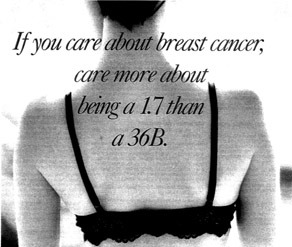
\includegraphics[width=2in]{nolvadexad_photo.jpg}}

\end{enumerate}



\end{multicols}